\section{Strangeness abundance in cosmic plasma}
\label{Strangeness}
%{Heavy-quark in primordial QGP: after hadronization}
As the Universe expanded and cooled down to the hadronization temperature $T_H\approx150$ MeV, the primordial QGP underwent a phase transformation called hadronization. This transition resulted in the confinement of the strong force, causing quarks and gluons to combine and form matter 
and antimatter. After hadronization, one may think the relatively short lived massive hadrons decay rapidly and disappear from the Universe. However, the most abundant hadrons, pions $\pi(q\bar q)$, can be produced via their inverse decay process $\gamma\gamma\rightarrow\pi^0$ and retain their chemical equilibrium until temperature $T=3\sim5$ MeV~\cite{Kuznetsova:2008jt}. 

Following the idea and the framework presented by~\cite{Kuznetsova:2008jt}, we investigate the strange particle composition of the expanding early Universe in the epoch $150\,\mathrm{MeV}\ge T\ge 10$\,MeV, and examine the freeze-out temperature for strangeness-producing  by comparing the relevant reaction rates to the Hubble expansion rate. We show that strangeness is kept in equilibrium via weak, electromagnetic, and strong interactions in the early Universe until $T\approx13$ MeV.


 
%~~~~~~~~~~~~~~~~~~~~~~~~~~~~~~~~~~~~~~~~~~~~~~~~~



%~~~~~~~~~~~~~~~~~~~~~~~~~~~~~~~~~~~~~~~~~~~~~~~~~

\subsection{Chemical equilibrium in the hadronic Universe}
%In this section we will focus on the following:
%\begin{itemize}
%    \item Chemical potentials of $\mu_B$ and $\mu_s$
%    \item Composition of universe (strangeness abundance)
%\end{itemize}

In this section, we explore the Universe composition assuming both kinetic and particle abundance equilibrium (chemical equilibrium) by considering the charge neutrality and prescribed conserved baryon-per-entropy-ratio ${(n_B-n_{\overline{B}})}/{\sigma}$ to determine the baryon chemical potential $\mu_B$~\cite{Fromerth:2012fe,Rafelski:2013yka}. With the chemical potential as a function of temperature, we can obtain the particle number densities for different species and study their composition in the early Universe.

We improve the prior work~\cite{Fromerth:2012fe} by considering the conserved entropy per baryon ratio with conservation of strangeness in the early Universe. To study the baryon and strange quark chemical potential, it is convenient to introduce the chemical fugacity for strangeness $\lambda_s$ and quark $\lambda_q$ as follows:\index{baryon chemical potential}
\begin{align}
\lambda_s=\exp(\mu_s/T)\,\quad \lambda_q=\exp(\mu_B/3T),
\end{align}
where $\mu_s$ and $\mu_B$ are the chemical potential of strangeness and baryon, respectively. For the quark fagucity $\lambda_q$, we divide the chemical potential of baryons by 3 as an approximation for quark chemical potential. Imposing the conservation of strangeness  
$\langle s-\bar s \rangle=0$, we have, when the baryon chemical potential does not vanish the chemical potential of strangeness in the early Universe satisfying (see Section 11.5 in \,\cite{Letessier:2002ony})\index{strange quark! chemical potential}
\begin{align}\label{museq}
\lambda_s=\lambda_q\sqrt{\frac{F_K+\lambda^{-3}_q\,F_Y}{F_K+\lambda^3_q\,F_Y}}.
\end{align}
where we employ the phase-space function $F_i$ for sets of nucleon $N$, kaon $K$, and hyperon $Y$ particles defined as (see \cite{Letessier:2002ony}, Section 11.4):
\begin{align}
&F_N=\sum_{N_i}\,g_{N_i}W(m_{N_i}/T)\;, \quad N_i=n, p, \Delta(1232),\\
&F_K=\sum_{K_i}\,g_{K_i}W(m_{K_i}/T)\;, \quad K_i=K^0, \overline{K^0}, K^\pm, K^\ast(892),\\
&F_Y=\sum_{Y_i}\,g_{Y_i}W(m_{Y_i}/T)\;, \quad Y_i=\Lambda, \Sigma^0,\Sigma^\pm, \Sigma(1385),
\end{align}
where $g_{N_i,K_i,Y_i}$ are the degenerate factors, $W(x)=x^2K_2(x)$ with $K_2$ is the modified Bessel functions of integer order "$2$".  

Considering the Boltzmann approximation for the massive particle number density we have
\begin{align}
\label{Density_N}
&n_N=\frac{T^3}{2\pi^2}\lambda_q^3F_N,\quad\qquad\qquad n_{\overline N}=\frac{T^3}{2\pi^2}\lambda^{-3}_qF_N,\\
\label{Density_K}
&n_K=\frac{T^3}{2\pi^2}\left(\lambda_s\lambda_q^{-1}\right)F_K,\,\qquad n_{\overline{K}}=\frac{T^3}{2\pi^2}\left(\lambda_s^{-1}\lambda_q\right)F_K,\\
\label{Density_Y}
&n_Y=\frac{T^3}{2\pi^2}\left(\lambda_q^2\lambda_s\right)F_Y,\quad\qquad n_{\overline Y}=\frac{T^3}{2\pi^2}\left(\lambda^{-2}_q\lambda_s^{-1}\right)F_Y.
\end{align}
In this case, the net baryon density in the early Universe with temperature range $150\,\mathrm{MeV}> T>10$\,MeV can be written as 
\begin{align}
\frac{\left(n_B-n_{\overline{B}}\right)}{\sigma}&=\frac{1}{\sigma}\left[\left(n_p-n_{\overline{p}}\right)+\left(n_n-n_{\overline{n}}\right)+\left(n_Y-n_{\overline{Y}}\right)\right]\notag\\
&=\frac{T^3}{2\pi^2\,\sigma}\left[\left(\lambda_q^3-\lambda^{-3}_q\right)F_N+\left(\lambda_q^2\lambda_s-\lambda^{-2}_q\lambda_s^{-1}\right)F_Y\right]\notag\\
&=\frac{T^3}{2\pi^2\sigma}\left(\lambda_q^3-\lambda_q^{-3}\right)F_N\left[1+\frac{\lambda_s}{\lambda_q}\left(\frac{\lambda_q^3-\lambda^{-1}_q\lambda_s^{-2}}{\lambda^3_q-\lambda^{-3}_q}\right)\,\frac{F_Y}{F_N}\right]\notag\\
&\approx\frac{T^3}{2\pi^2\sigma}\left(\lambda_q^3-\lambda_q^{-3}\right)F_N\left[1+\frac{\lambda_s}{\lambda_q}\,\frac{F_Y}{F_N}\right],
\end{align}
where we can neglect the term $F_Y/F_K$ in the expansion of Eq.(\ref{museq}) in our temperature range. Introducing the strangeness $\langle s-\bar s\rangle=0$ constraint and using the entropy density in early universe, the explicit relation for baryon to entropy ratio becomes
\begin{align}\label{muBeq}
\frac{n_B-n_{\overline{B}}}{\sigma}&=\frac{45}{2\pi^4g^s_\ast}\sinh\left[\frac{\mu_B}{T}\right]F_N\times\left[1+\frac{F_Y}{F_N}\sqrt{\frac{1+e^{-\mu_B/T}\,F_Y/F_K}{1+e^{\mu_B/T}\,F_Y/F_K}}\right].
\end{align}
Governing Eq.\,(\ref{muBeq}) is the present-day baryon-per-entropy-ratio, and we obtain the value 
\begin{align}\label{BdS}
\frac{n_B-n_{\overline{B}}}{\sigma}= \left.\frac{n_B-n_{\overline{B}}}{ \sigma}\right|_{t_0}=(0.865\pm0.008)\times10^{-10} \;.
\end{align}
For a detailed evaluation method we refer to this earlier work now using a baryon-to-photon ratio~\cite{ParticleDataGroup:2018ovx}: $\left(n_B-n_{\overline{B}}\right)/n_\gamma= (0.609\pm0.06)\times10^{-9}$, as well as the entropy per particle for a massless boson $\sigma/n|_\mathrm{boson}\approx 3.60$ and a massless fermion $\sigma/n|_\mathrm{fermion}\approx 4.20$. 

%~~~~~~~~~~~~~~~~~~~~~~~~~~~~~~~~~~~~~~~~~~~~~~~~~~~~~~~~~~~~~~~~~~~~~~~~~~~~~~~~
\begin{figure}[t]
%\begin{center}
\centering
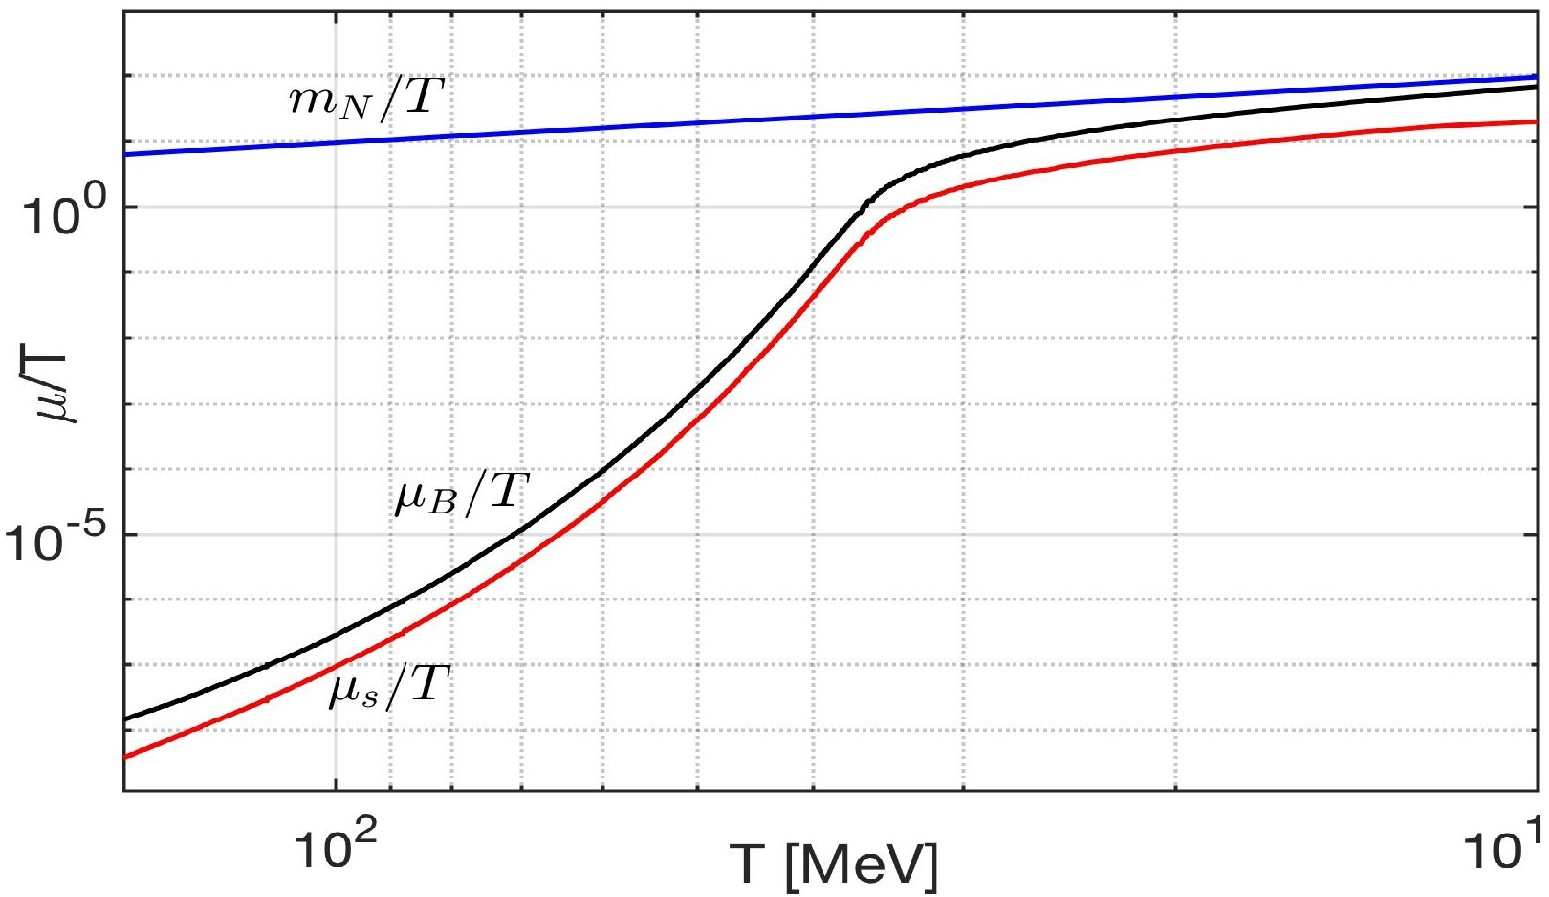
\includegraphics[width=\textwidth]{./plots/New_Chemical_Potential_C.jpg}
\caption{\cccite{Yang:2021bko}, adapted from thesis of C.T.Yang \cite{Yang:2024ret}. The chemical potential of baryon $\mu_B/T$ and strangeness $\mu_s/T$ as a function of temperature $150\,\mathrm{MeV}> T>10\,\mathrm{MeV}$ in the early Universe; for comparison we show $m_N/T $ with $m_N=938.92$\,MeV, the average nucleon mass.}
\label{ChemPotFig}
%\end{center}
\end{figure}
%~~~~~~~~~~~~~~~~~~~~~~~~~~~~~~~~~~~~~~~~~~~~~~~~~~~~~~~~~~~~~~~~~~~~~~~~~~~~~~
%%%%%%%%%%%%%%%%%%%%%%%%%%%%%%%%%%%%%%%
\begin{figure}[h]
\centering
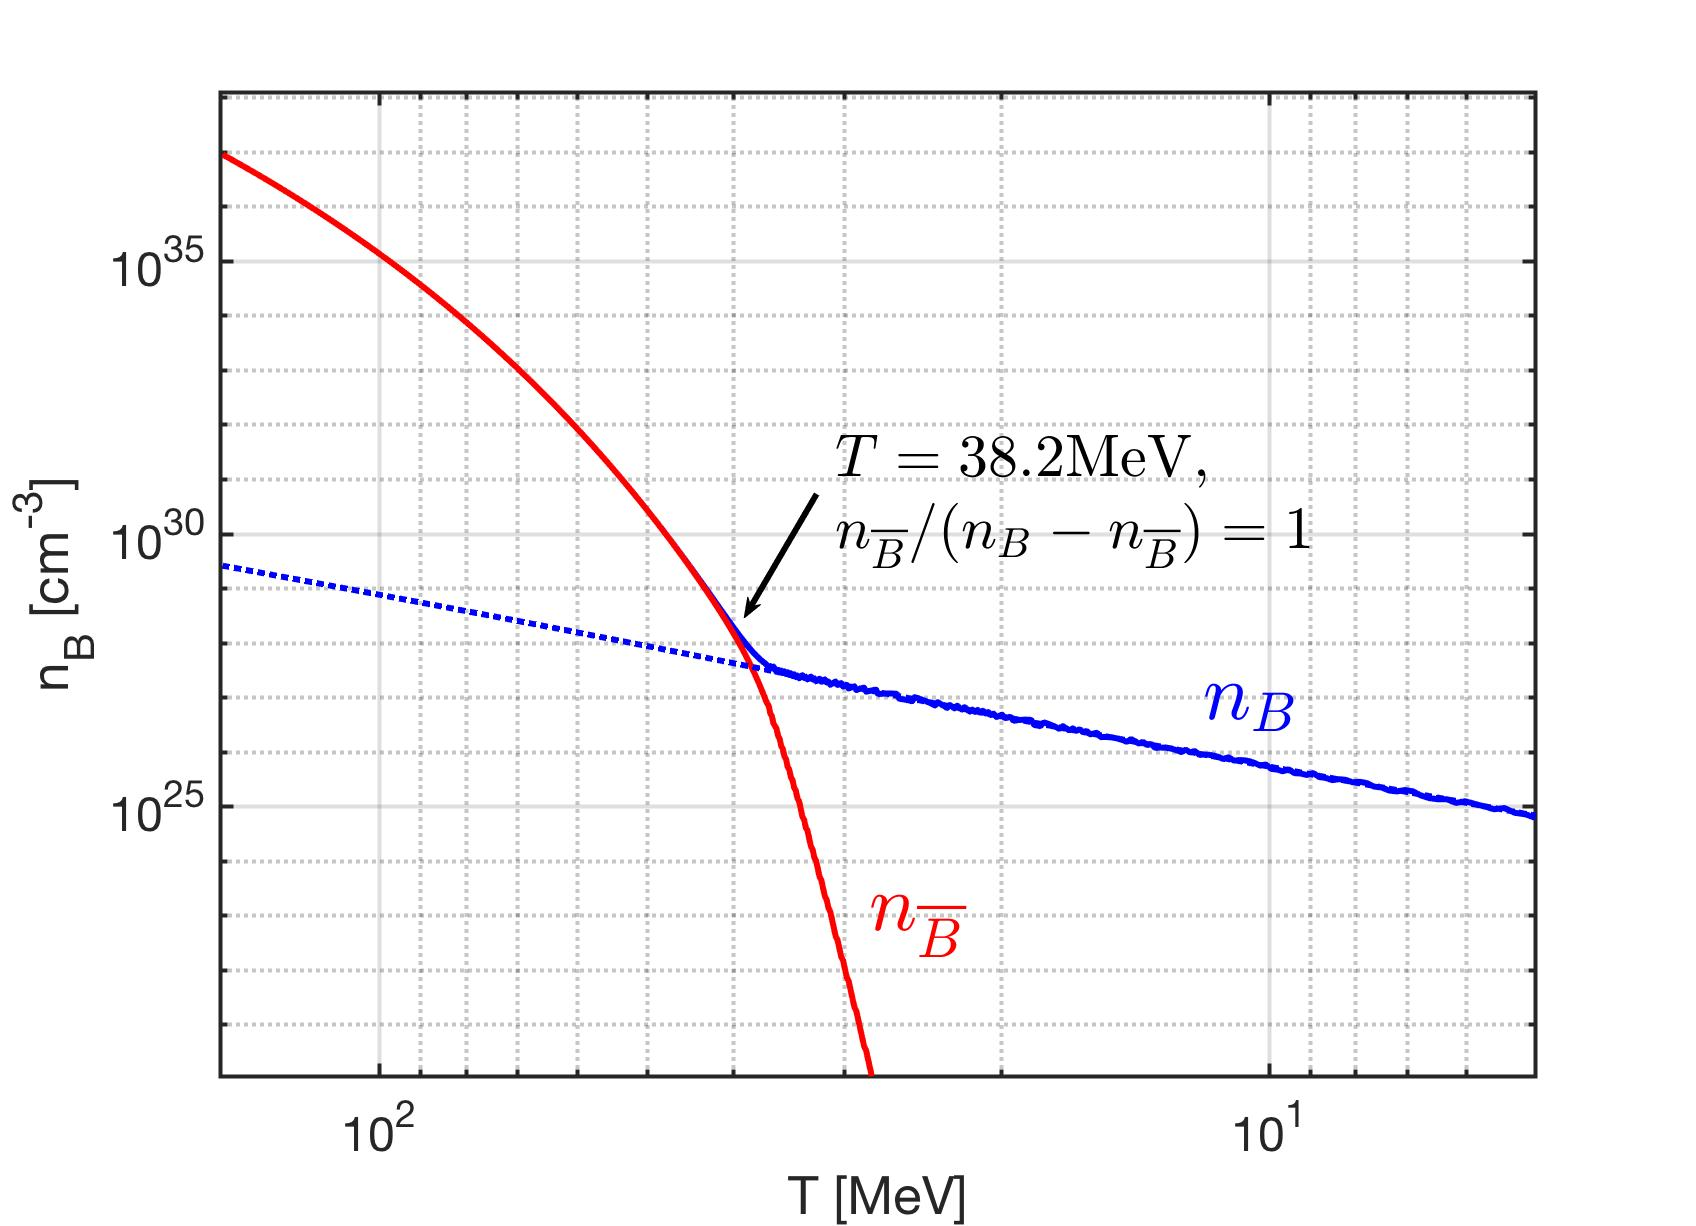
\includegraphics[width=\textwidth]{./plots/Baryon_Antibaryon_cm.jpg}
\caption{\cccite{Rafelski:2023emw}, adapted from thesis of C.T.Yang \cite{Yang:2024ret}. The baryon (blue solid line) and antibaryon (red solid line) number density as a function of temperature in the range $150\,\mathrm{MeV}>T>5\,\mathrm{MeV}$. The blue dotted line is the extrapolated value for baryon density. The temperature $T=38.2\,\mathrm{MeV}$ is denoted when the ratio $n_{\overline B}/(n_B-n_{\overline B})=1$ which defines the condition where antibaryons disappear from the Universe.}
\label{Baryon_fig}
\end{figure}
%%%%%%%%%%%%%%%%%%%%%%%%%%%%%%%%%%%%%%%


We solve Eq.~(\,\ref{museq}) and Eq~(\ref{muBeq}) numerically to obtain baryon and strangeness chemical potentials as a function of temperature in Fig.~\ref{ChemPotFig}. The chemical potential changes dramatically in the temperature window $50\,\mathrm{MeV}\le T\le 30$\,MeV, its behavior describing the process of antibaryon disappearance. Substituting the chemical potential $\lambda_q$ and $\lambda_s$ into particle density Eq.~(\ref{Density_N}), Eq.~(\ref{Density_K}), and Eq.~(\ref{Density_Y}), we can obtain the particle number densities for different species as a function of temperature.

In Fig.~\ref{Baryon_fig} we plot the number density of baryon and antibaryon as a function of temperature. We consider that when the  $n_{\overline B}\ll(n_B-n_{\overline B})$ the anitbaryons density is sufficient low and disappear from the Universe inventory quickly. To determine the temperature where antibaryons is sufficient law in the Universe inventory we defined the condition when the ratio $n_{\overline B}/(n_B-n_{\overline B})=1$. This condition is reached in an expanding Universe at $T=38.2$\,MeV, which is in agreement with the qualitative result in \cite{Kolb:1990vq}. After this temperature, the net baryon density dilutes with a residual co-moving conserved quantity determined by the observed baryon asymmetry.



%~~~~~~~~~~~~~~~~~~~~~~~~~~~~~~~~~~~~~~~~~~~~~~~~~~~~~~~~~~~~~~~~~~~~~~~~~~~~~~~~
\begin{figure}[bt]
%\begin{center}
\centering
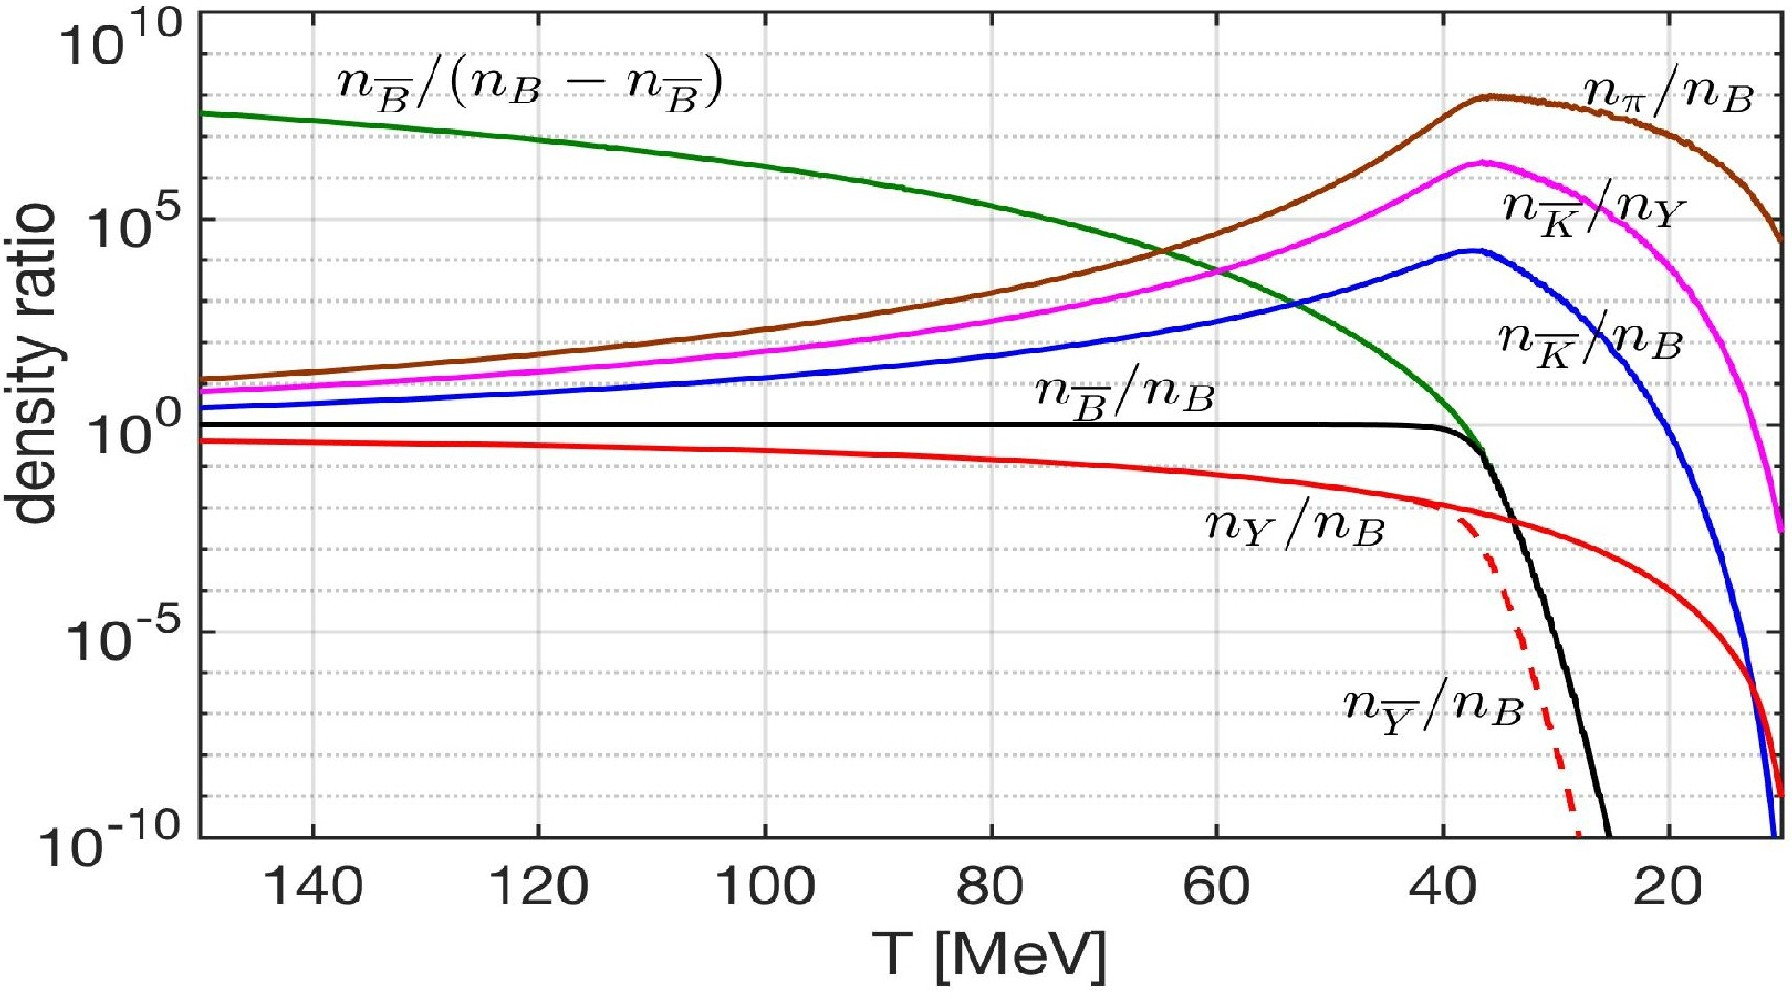
\includegraphics[width=\textwidth]{./plots/Meson_Baryon_density_ratio_C.jpg}
\caption{\cccite{Rafelski:2023emw}, adapted from Ref.~\cite{Yang:2021bko} and thesis of C.T.Yang \cite{Yang:2024ret}. Ratios of hadronic particle number densities as a function of temperature $150\,\mathrm{MeV}> T>10\,\mathrm{MeV}$ in the early Universe, with baryon $B$ yields: pions $\pi$ (brown line), kaons $K( q\bar s)$ (blue), antibaryon $\overline B$ (black), hyperon $Y$ (red) and anti-hyperons $\overline Y$ (dashed red). Also shown $\overline K/Y$(purple).}
\label{EquilibPartRatiosFig}
%\end{center}
\end{figure}
%~~~~~~~~~~~~~~~~~~~~~~~~~~~~~~~~~~~~~~~~~~~~~~~~~~~~~~~~~~~~~~~~~~~~~~~~~~~~~~

In Fig.~\ref{EquilibPartRatiosFig} we show examples of particle abundance ratios of interest\index{hadron density}. %Considering $n_Y/n_B$ we see that hyperons $Y(sqq)$ remain a noticeable 1\% component in baryon yield through this domain of antibaryon decoupling.
Pions $\pi(q\bar q)$ are the most abundant hadrons $n_\pi/n_B\gg1$, because of their low mass and the reaction $\gamma\gamma\rightarrow\pi^0$, which assures chemical yield equilibrium~\cite{Kuznetsova:2008jt}. For $150\,\mathrm{MeV}>T>20.8\,\mathrm{MeV}$, we see the ratio $n_{{\overline K}(\bar q s)}/n_B\gg1$, which implies pair abundance of strangeness is more abundant than baryons, and is dominantly present in mesons, since $n_{\overline K}/n_Y\gg1$. 
For $20.8\,\mathrm{MeV}>T$, the baryon becomes dominant $n_{\overline K}/n_B<1$, which implies that the strange meson is embedded in a large background of baryons, and the exchange reaction $\overline{K}+N\rightarrow \Lambda+\pi$ can re-equilibrate kaons and hyperons in the temperature range; therefore strangeness symmetry $s=\bar s$ is maintained. For $12.9\,\mathrm{MeV}>T$ we have $n_Y/n_B>n_{\overline K}/n_B$, now the still existent tiny abundance of strangeness is found predominantly in hyperons.


%~~~~~~~~~~~~~~~~~~~~~~~~~~~~~~~~~~~~~~~~~~~~~~~~~

%~~~~~~~~~~~~~~~~~~~~~~~~~~~~~~~~~~~~~~~~~~~~~~~~~

\subsection{Seeking strangeness freeze-out chemical nonequilibrium
}
%In this section we will focus on the following:
%\begin{itemize}
%    \item Relevant strangeness reactions
%    \item Strangeness creation/annihilation in mesons
%    \item Strangeness production/ exchange in hyperons
%    \item Strangeness epochs in  the Universe 
%\end{itemize}

%In this section, we focus on investigating the strangeness abundance and decoupling following the formation of normal matter during the hadronization process of the quark-gluon plasma (QGP). Nonequilibrium conditions in the early Universe are of general interest: they are understood to be prerequisite for the arrow of time dependent processes to take hold in the Hubble expanding Universe.
%~~~~~~~~~~~~~~~~~~~~~~~~~~~~~~~~~~~~~~~~~~~~~~~~~~~~~~~~~~~~

%\subsection{Relevant strangeness reactions}
This section considers an unstable strange particle $S$ decaying into two particles $1$ and $2$, which themselves have no strangeness content. In a dense and high-temperature plasma with particles $1$ and $2$ in thermal equilibrium, the inverse reaction populates the system with particle $S$. This is written schematically as
\begin{align}
 S\Longleftrightarrow1+2,\qquad \mathrm{Example}: K^0\Longleftrightarrow\pi+\pi\,.
\end{align}
The natural decay of the daughter particles provides the intrinsic strength of the inverse strangeness production reaction rate. As long as both decay and production reactions are possible, particle $S$ abundance remains in thermal equilibrium. This balance between production and decay rates is called a detailed balance.

Once the primordial Universe expansion rate $1/H$ overwhelms the strongly temperature dependent back-reaction and the back reaction freeze-out, then the decay $S\rightarrow 1+2$ occurs out of balance and particle $S$ disappears from the inventory. The two-on-two strangeness producing reactions have a significantly higher strangeness production reaction threshold, thus especially near to strangeness decoupling their influence is negligible. Such reactions are more important near the QGP hadronization temperature $T_H\simeq 150$\,MeV, and they characterize strangeness exchange reactions such as $\mathrm{K}+N\leftrightarrow \Lambda+\pi$, (see Chapter 18 in \cite{Letessier:2002ony}).


In Fig.~\ref{Strangeness_map2} we show reactions relevant to strangeness evolution in the considered Universe evolution epoch $150\,\mathrm{MeV}\ge T\ge 10$\,MeV  and their pertinent reaction strength. As shown:
\begin{itemize}
\item
We study strange quark abundance in baryons and mesons, considering both open and hidden strangeness (hidden: $s\bar s$-content). Important source reactions are $l^-+l^+\rightarrow\phi$, $\rho+\pi\rightarrow\phi$, $\pi+\pi\rightarrow K_\mathrm{S}$, $\Lambda \leftrightarrow \pi+ N$, and $\mu^\pm+\nu\rightarrow K^\pm$. 
\item
Muons and pions are coupled through electromagnetic reactions $\mu^++\mu^-\leftrightarrow\gamma+\gamma$ and $\pi\leftrightarrow\gamma+\gamma$ to the photon background and retain their chemical equilibrium until the temperature $T =4$\, MeV and $T=5$\,MeV, respectively~\cite{Rafelski:2021aey,Kuznetsova:2008jt}. The large $\phi\leftrightarrow K+K$ rate assures $\phi$ and $K$ are in relative chemical equilibrium.
\end{itemize}
In order to determine where exactly strangeness disappears from the Universe inventory, we explore the magnitudes of different rates of production and decay processes in mesons and hyperons.
%~~~~~~~Figure~~~~~~~~~~~~~~~~~~~~~~~~~~~~~~~~~~~~~~~~~~~~~~~~~~~~~~~~~~~~~~~~~~~~
\begin{figure} %[h]
%\begin{center}
\centering
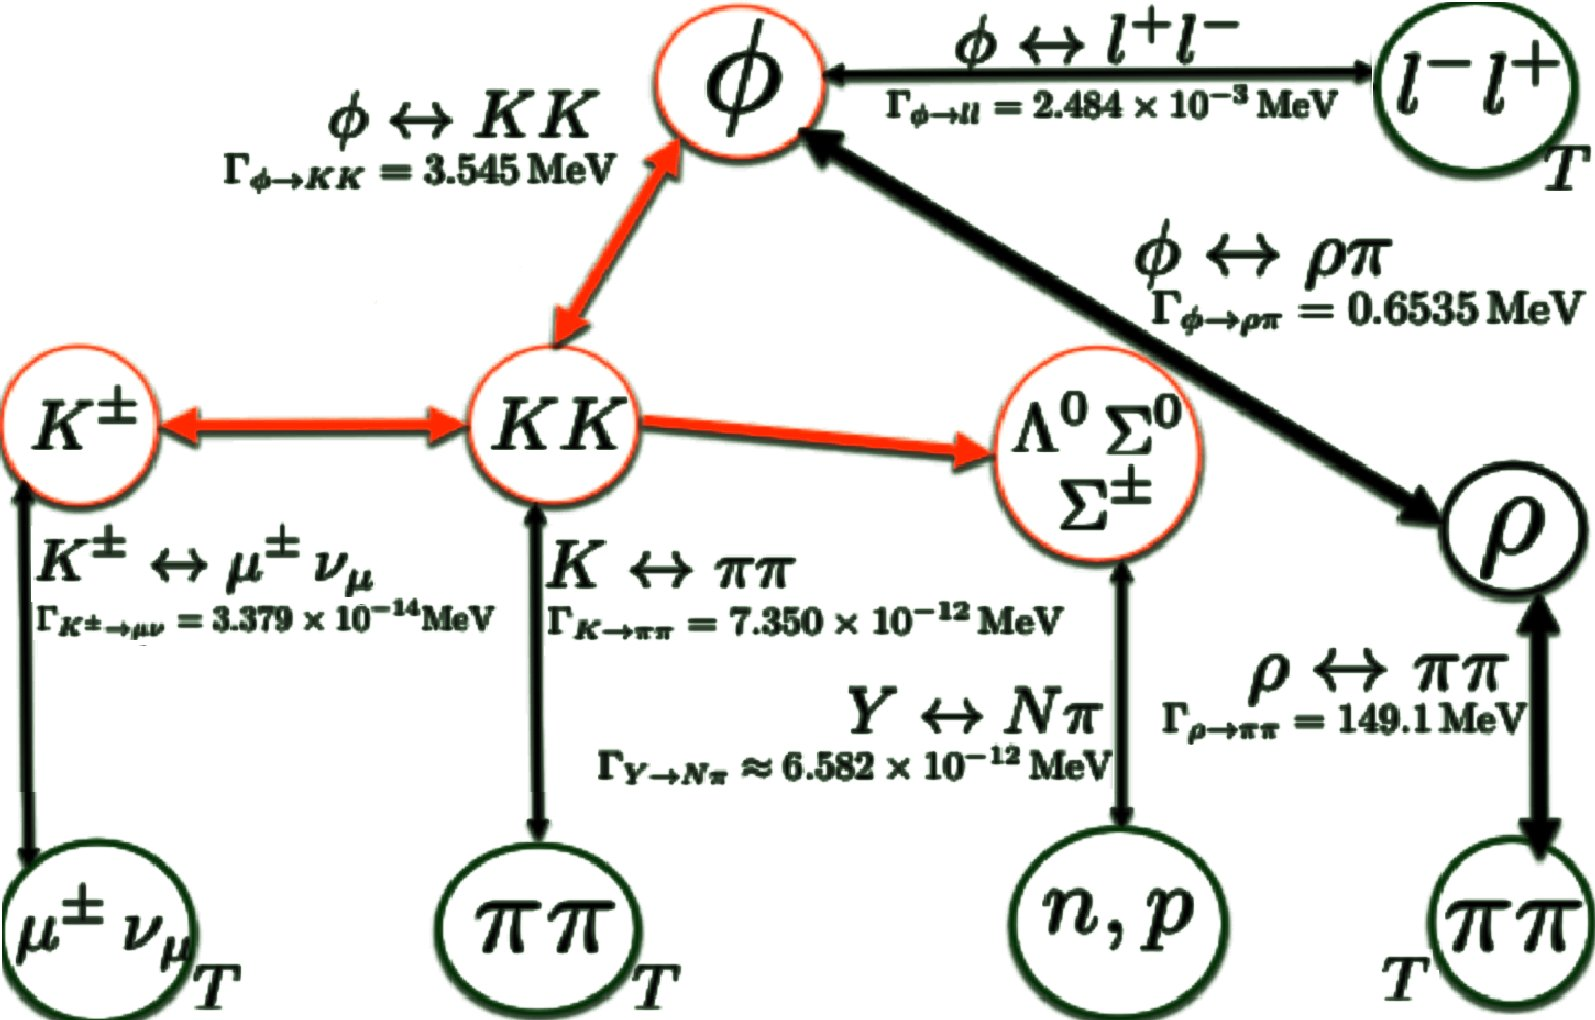
\includegraphics[width=0.75\linewidth]{./plots/Strangeness002_newJ.jpg}
\caption{\cccite{Rafelski:2023emw}, adapted from Ref.~\cite{Yang:2021bko} and thesis of C.T.Yang \cite{Yang:2024ret}. The strangeness abundance changing reactions in the primordial Universe. The red circles show strangeness carrying hadronic particles; red thick lines denote effectively instantaneous reactions. Black thick lines show relatively strong hadronic reactions. The reaction rates required to describe  strangeness time evolution are shown in \cite{Rafelski:2020ajx}.
}
\label{Strangeness_map2}
%\end{center}
\end{figure}
%~~~~~~~~~~~~~~~~~~~~~~~~~~~~~~~~~~~~~~~~~~~~~~~~~~~~~~~~~~~~~~~~~~~~~~~~~~



\subsection{Strangeness creation/annihilation rate in mesons}
From Fig.~\ref{Strangeness_map2} in the meson domain, the relevant interaction rates competing with Hubble time are the reactions\index{strange quark! mesons production rate}
\begin{align}
 &\pi+\pi\leftrightarrow K\,,\quad\mu^\pm+\nu\leftrightarrow K^\pm\,,\quad l^++l^-\leftrightarrow\phi\,,\\
 &\rho+\pi\leftrightarrow\phi\,,\quad \pi+\pi\leftrightarrow\rho\,.
\end{align}
The thermal reaction rate per time and volume for two body-to-one particle reactions $1+2\rightarrow 3$ has been presented before~\cite{Koch:1986ud,Kuznetsova:2008jt,Kuznetsova:2010pi}. In full kinetic and chemical equilibrium, the reaction rate per time per volume can be written as~\cite{Kuznetsova:2010pi} :\index{inverse decay rate}
\begin{align}
&R_{12\to 3}=\frac{g_3}{(2\pi)^2}\,\frac{m_3}{\tau^0_3}\,\int^\infty_0\frac{p^2_3dp_3}{E_3}\frac{e^{E_3/T}}{e^{E_3/T}\pm1}\Phi(p_3)\;,
\end{align}
where $\tau^0_3$ is the vacuum lifetime of particle $3$. The positive sign $``+"$ is for the case when particle $3$ is a boson, and negative sign $``-"$ for fermion. The function $\Phi(p_3)$ for the non-relativistic limit $m_3\gg p_3,T$ can be written as 
\begin{align}
\Phi(p_3\to0)=2\frac{1}{(e^{E_1/T}\pm1)(e^{E_2/T}\pm1)}.
\end{align}


Considering the Boltzmann limit, the thermal reaction rate per unit time and volume becomes
\begin{align}
\label{Thermal_Rate}
R_{12\rightarrow3}=\frac{g_3}{2\pi^2}\left(\frac{T^3}{\tau^0_3}\right)\left(\frac{m_3}{T}\right)^2\,K_1(m_3/T),
\end{align}
where $K_1$ is the modified Bessel functions of integer order "$1$". In order to compare the reaction time with Hubble time $1/H$, it is convenient to define the relaxation time for the process $1+2\rightarrow 3$ as follows:
\begin{align}
\label{Reaction_Time}
\tau_{12\rightarrow 3}\equiv\frac{n^{eq}_{1}}{R_{12\rightarrow n}}\,,\quad
n^{eq}_1=\frac{g_1}{2\pi^2}\int_{m_1}^\infty\!\!\!\!dE\,\frac{E\,\sqrt{E^2-m_1^2}}{\exp{\left(E/T\right)}\pm1}\;, 
\end{align}
where $n^{eq}_1$\,is the thermal equilibrium number density of particle\,$1$ with the `heavy' mass $m_1>T$.  Combining Eq.\,(\ref{Thermal_Rate}) with  Eq.\,(\ref{Reaction_Time}) we obtain
\begin{align}\label{RelaxationTime}
&\frac{\tau_{12\rightarrow3}}{ \tau^0_3}=  
\frac{2\pi^2 n^{eq}_1/T^3}{g_3(m_3/T)^2\,K_1(m_3/T)}\,, \quad 
n^{eq}_1\simeq g_1\left(\frac{m_1 T}{2\pi}\right)^{3/2}e^{-m_1/T},
\end{align}
where, conveniently, the relaxation time does not depend on the abundant and often relativistic heat bath component $2$, {\it e.g.\/} $l^\pm,\pi,\nu,\gamma$. The density of heavy particles\,$1$\,and\,$3$ can in general be well approximated using the leading and usually nonrelativistic Boltzmann term as shown above.

In general, the reaction rates for inelastic collision process capable of changing particle number, for example $\pi\pi\to K^0$, is suppressed by the factor $\exp{(-m_{K^0}/T)}$. On the other hand, there is no suppression for the elastic momentum and energy exchanging particle collisions in plasma. We conclude that for the case $m\gg T$, the dominant collision term in the relativistic Boltzmann equation is the elastic collision term, keeping all heavy particles in kinetic energy equilibrium with the plasma. This allows us to study the particle abundance in plasma presuming the energy-momentum statistical distribution equilibrium exists. This insight was discussed in detail in the preparatory phase of laboratory exploration of hot hadron and quark matter, see~\cite{Koch:1986ud}. In order to study the particle abundance in the Universe when $m\gg T$, instead of solving the exact Boltzmann equation, we can separate the fast energy-momentum equilibrating collisions from the slow particle number changing inelastic collisions. In the following we explore the rates of inelastic collision and compare the relaxation times of particle production in all relevant reactions with the Universe expansion rate.



It is common to refer to particle freeze-out as the epoch where a given type of particle ceases to interact with other particles. In this situation the particle abundance decouples from the cosmic plasma, a chemical nonequilibrium and even complete abundance disappearance of this particle can happen; the condition for the given reaction $1+2\rightarrow 3$ to decouple is
\begin{align}
\tau_{12\rightarrow 3}(T_f)=1/H(T_f),
\end{align}
where $T_f$ is the freeze-out temperature.
In the epoch of interest, $150\,\mathrm{MeV}>T>10\,\mathrm{MeV}$, the Universe is dominated by radiation and effectively massless matter behaving like radiation. The Hubble parameter can be written as~\cite{Kolb:1990vq}
\begin{align}\label{H2g}
H^2=H^2_{rad}\left(1+\frac{\rho_{\pi,\,\mu,\,\rho}}{\rho_\mathrm{rad}}+\frac{\rho_\mathrm{strange}}{\rho_\mathrm{rad}}\right)=\frac{8\pi^3G_\mathrm{N}}{90}g^e_\ast T^4,\qquad H^2_\mathrm{rad}=\frac{8\pi G_\mathrm{N}\,\rho_\mathrm{rad}}{3},
\end{align}
where: $g^e_\ast$ is the total number of effective relativistic `energy' degrees of freedom; $G_\mathrm{N}$ is the Newtonian constant of gravitation; the `radiation' energy density includes $\rho_\mathrm{rad}=\rho_\gamma+\rho_\nu+\rho_{e^\pm}$ for photons, neutrinos, and massless electrons(positrons). The massive-particle correction is $\rho_{\pi,\,\mu,\,\rho}=\rho_\pi+\rho_\mu+\rho_\rho$; and at highest $T$ of interest, also of (minor) relevance, $\rho_\mathrm{strange}=\rho_{K^0}+\rho_{K^\pm}+\rho_{K^\ast}+\rho_{\eta}+\rho_{\eta^\prime}$.
%~~~~~~~Figure~~~~~~~~~~~~~~~~~~~~~~~~~~~~~~~~~~~~~~~~~~~~~~~~~~~~~~~~~~~~~~~~~~~~~~~~~~
\begin{figure}[ht]
%\begin{center}
\centering
%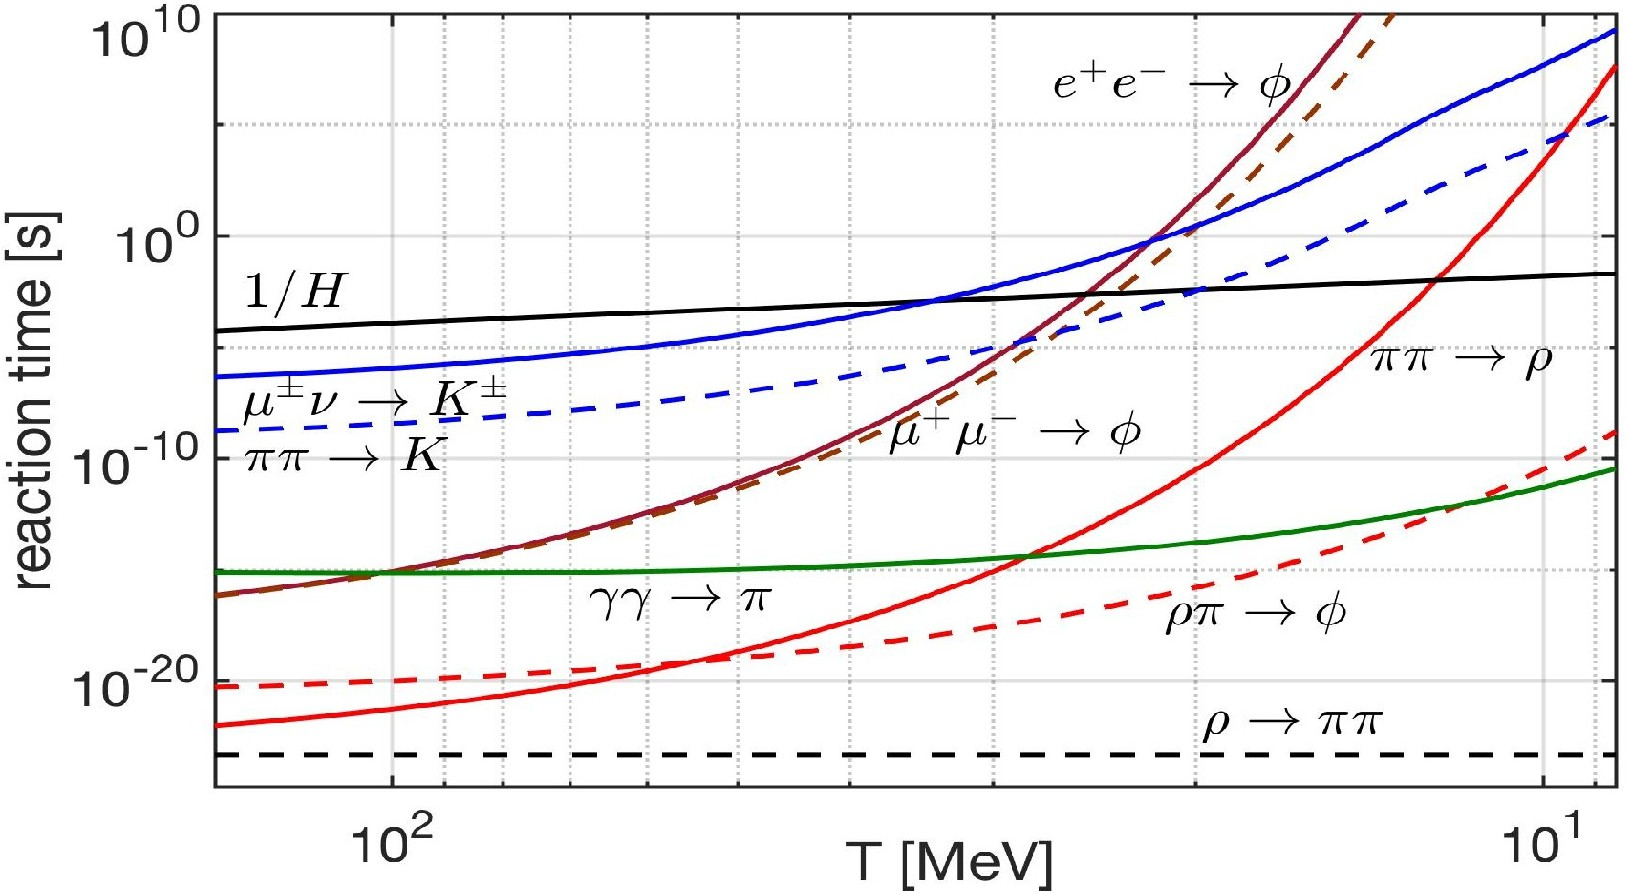
\includegraphics[width=0.95\linewidth]{./plots/Strangeness_Hubble_C.jpg}
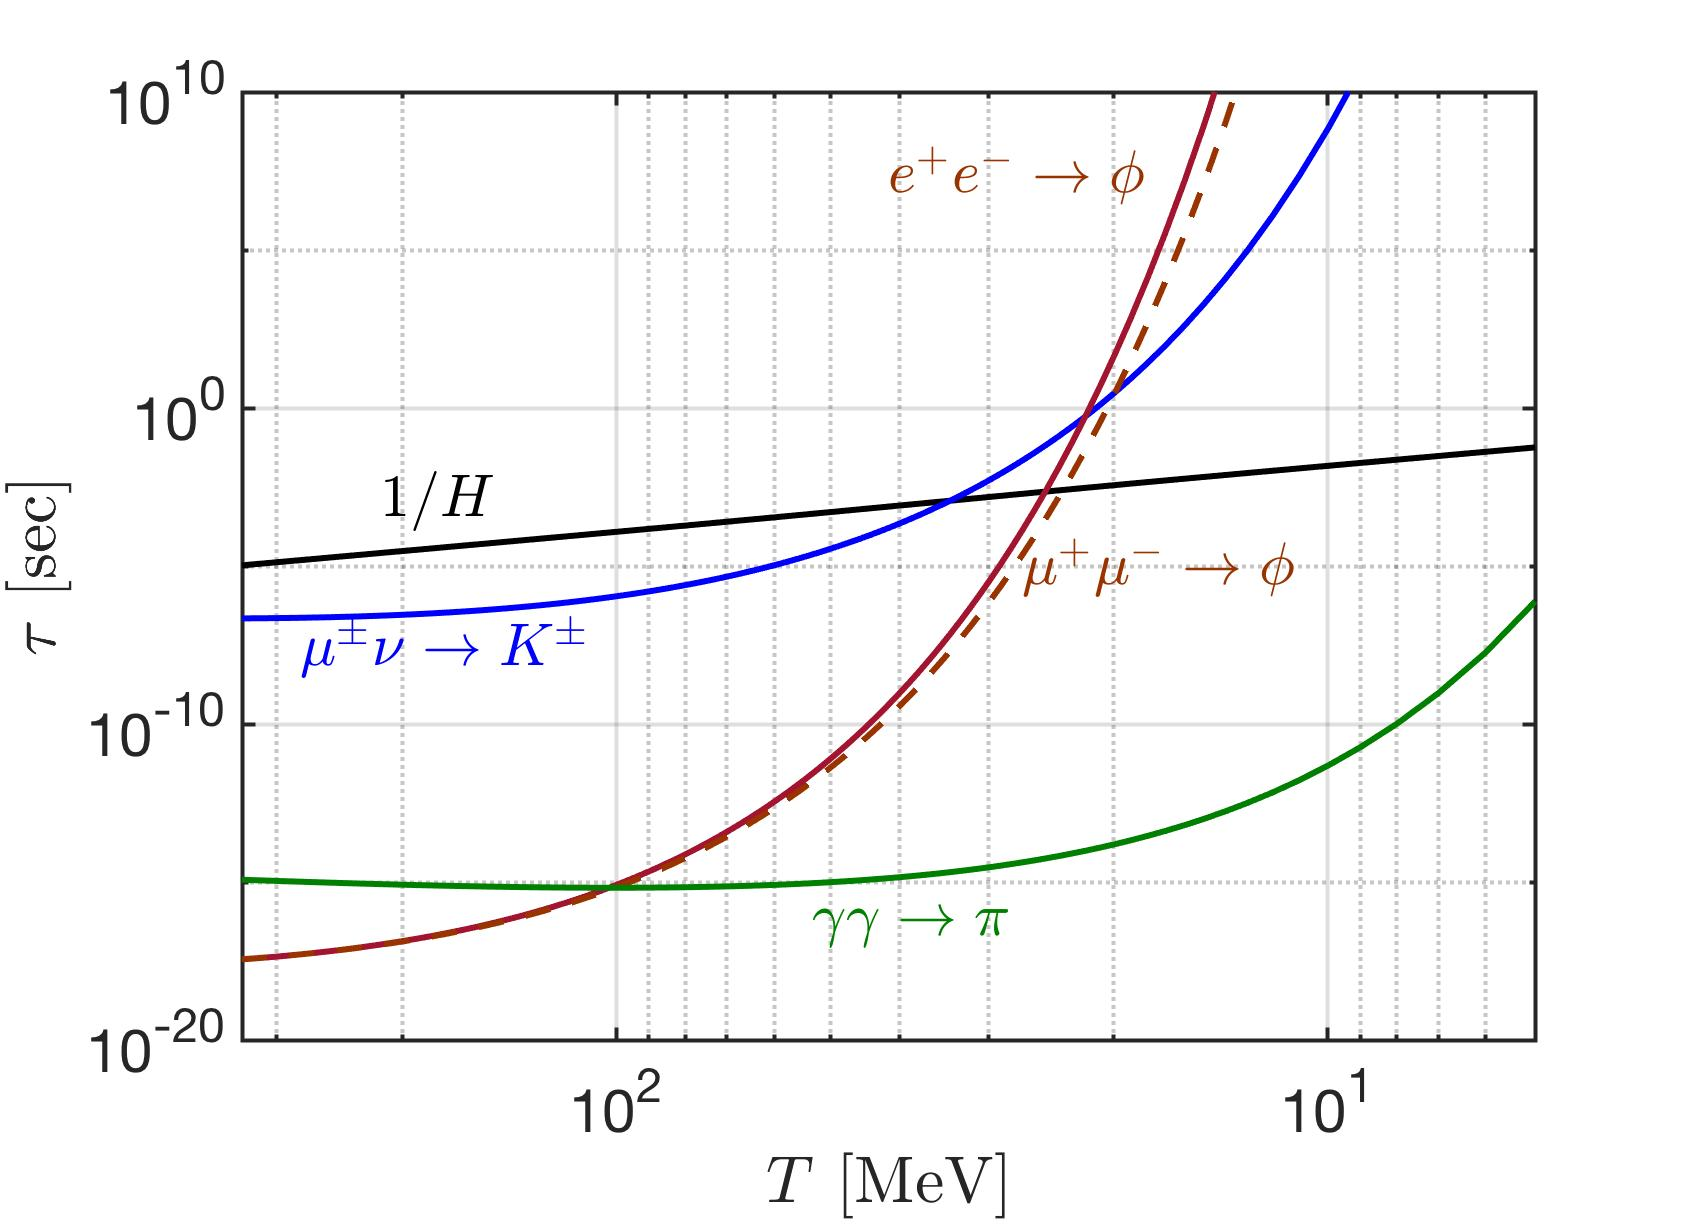
\includegraphics[width=1\linewidth]{./plots/Strangeness_Hubble002.jpg}
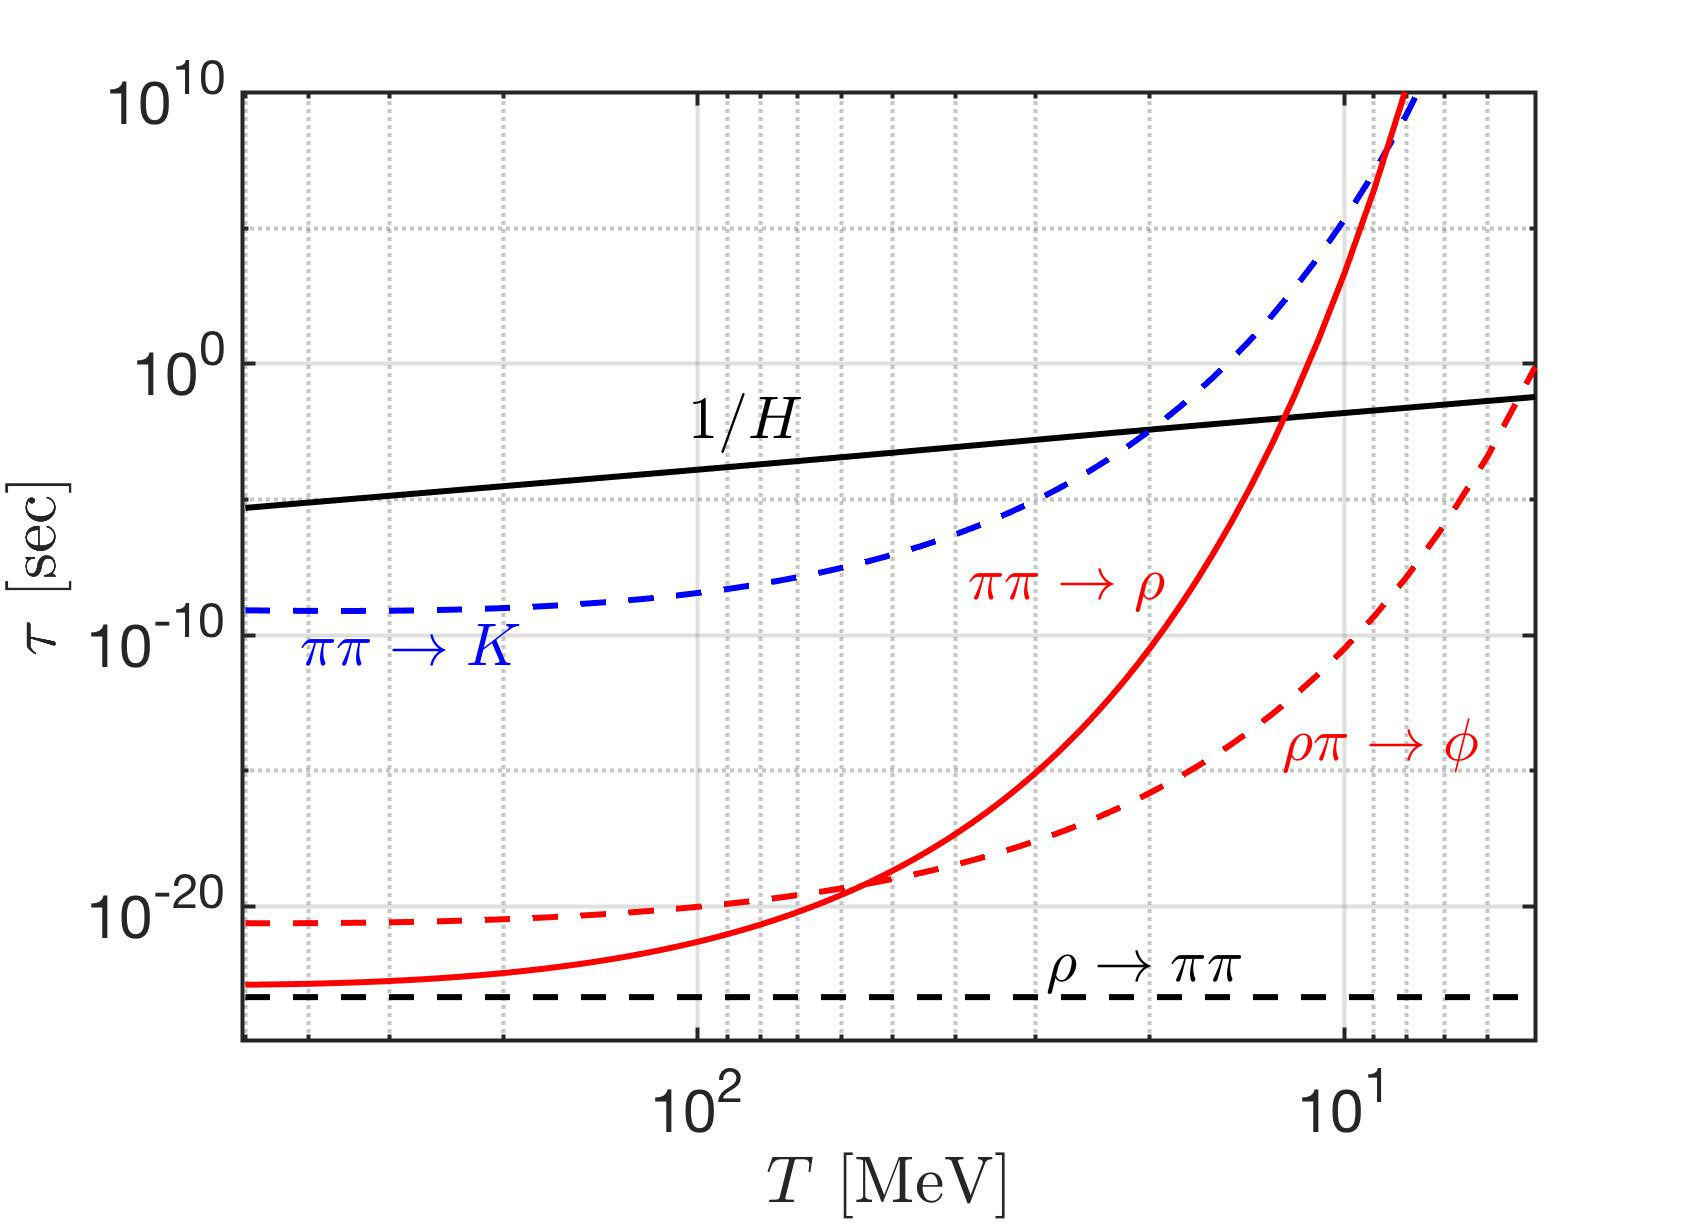
\includegraphics[width=1\linewidth]{./plots/Strangeness_Hubble003.jpg}
\caption{\cccite{Rafelski:2023emw}, adapted from Ref.~\cite{Yang:2021bko} and thesis of C.T.Yang \cite{Yang:2024ret}. Hadronic relaxation reaction times, see Eq.\,(\ref{Reaction_Time}), as a function of temperature $T$, are compared to Hubble time $1/H$ (black solid line). At bottom the horizontal black-dashed line is the natural (vacuum) lifespan of $\rho$.}
\label{reaction_time_tot}
%\end{center}
\end{figure}
%~~~~~~~~~~~~~~~~~~~~~~~~~~~~~~~~~~~~~~~~~~~~~~~~~~~~~~~~~~~~~~~~~~~~~~~~~~~~~~~~~~~~~


When presenting the reaction rates and quoting decoupling as a function of temperature $T$, we must remember that for a temperature range $50\,\mathrm{MeV}>T>5$\,MeV, we have $10^{-1}<dT/dt<10^{-4}$\,MeV/$\mu$s. We estimate the width of freezeout temperature interval $\Delta T_f$  as follows:
\begin{align}
\frac{1}{\Delta T_f}\equiv \left[\frac{1}{(\Gamma_{12\to3}/H)}\frac{d(\Gamma_{12\to3}/H)}{dT}\right]_{T_f},\quad \Gamma_{12\to3}\equiv\frac{1}{\tau_{12\to3}}.
\end{align}
Using Eq.(\ref{H2g}) and Eq.(\ref{RelaxationTime}) and considering the temperature range $50\,\mathrm{MeV}>T>5$\,MeV with $g^e_\ast\approx\mathrm{constant}$ we obtain using the Boltzmann approximation to describe the  massive particles\,$1$\,and\,$3$
\begin{align}\label{DeltaFreezeout}
 \frac{\Delta T_f}{ T_f} \approx\frac{T_f  }{ m_3 - m_1 -2T_f}\,,\quad m_3 - m_1>> T_f\,.
\end{align}
The width of freeze-out is shown in the right column in Table~\ref{FreezeoutTemperature_table}. We see a range of $2$-$10\%$. Therefore it is justified to consider as a decoupling condition in time the value of temperature at which the pertinent rate cross the Hubble expansion rate, see Fig.~\ref{reaction_time_tot}.
 
In Fig.~\ref{reaction_time_tot} we plot the  hadronic reaction relaxation times $\tau_{i}$ in the meson sector as a function of temperature compared to Hubble time $1/H$.
It shows that the weak interaction reaction $\mu^\pm+\nu_{\mu}\rightarrow K^\pm$ becomes slower compared to the Universe expansion near temperature $T_f^{K^\pm}=33.8\,\mathrm{MeV}$, signaling the onset of abundance nonequilibrium for $K^\pm$. For $T<T_f^{K^\pm}$, the reactions $\mu^\pm+\nu_{\mu}\rightarrow K^\pm$ decouples from the cosmic plasma; the corresponding detailed balance can be broken and the decay reactions $K^\pm\rightarrow\mu^\pm+\nu_{\mu}$ are acting like a (small) ``hole'' in the strangeness abundance ``pot''. If other strangeness production reactions did not exist, strangeness would disappear as the Universe cools below $T_f^{K^\pm}$. However, we have other reactions: $l^++l^-\leftrightarrow\phi$, $\pi+\pi\leftrightarrow K$, and $\rho+\pi\leftrightarrow\phi$ can still produce the strangeness in cosmic plasma and the rate is very large compared to the weak interaction decay.
%~~~~~~~~~~~~~~~~~~~~~~~~~~~~~~~~~~~~~~~~~~~~~~~~~~~~~~~~~~~~~~~~~~~~~~~~~~~~~~~~~~~~~~~~~
\begin{table}%[h]
\centering
\begin{tabular}{c| c| c}
\hline\hline
Reactions &Freeze-out Temperature (MeV) & {$\Delta T_f$\,(MeV)} \\
\hline
$\mu^\pm\nu\rightarrow K^\pm$ & $T_f=33.8$\,MeV & {$3.5$ \,MeV}\\ 
\hline
$e^+e^-\rightarrow \phi$ & $T_f=24.9$\,MeV &{$0.6$\,MeV}\\
$\mu^+\mu^-\rightarrow\phi$ & $T_f=23.5$\,MeV &{$0.6$\,MeV}\\
\hline
 $\pi\pi\rightarrow K$ & $T_f=19.8$\,MeV&{$1.2$\,MeV}\\
\hline
$\pi\pi\rightarrow\rho$ & $T_f=12.3$\,MeV&{$0.2$\,MeV}\\
\hline\hline
\end{tabular}
\caption{The characteristic strangeness reaction and their freeze-out temperature and temperature width in early Universe.}
\label{FreezeoutTemperature_table} 
\end{table}

%~~~~~~~~~~~~~~~~~~~~~~~~~~~~~~~~~~~~~~~~~~~~~~~~~~~~~~~~~~~~~~~~~~~~~~~~~ 

In Table~\ref{FreezeoutTemperature_table} we show the characteristic strangeness reactions and their freeze-out temperatures in the early Universe. The intersection of strangeness reaction times with $1/H$ occurs for $l^-+l^+\rightarrow\phi$ at $T_f^\phi=25\sim23\,\mathrm{MeV}$, and for $\pi+\pi\rightarrow K$ at $T_f^K=19.8\,\mathrm{MeV}$, for $\pi+\pi\rightarrow\rho$ at $T_f^\rho=12.3\,\mathrm{MeV}$. The reactions $\gamma+\gamma\rightarrow\pi$ and $\rho+\pi\leftrightarrow\phi$ are faster compared to $1/H$. However, the $\rho\to\pi+\pi$ lifetime (black dashed line in Fig.~\ref{reaction_time_tot}) is smaller than the reaction $\rho+\pi\leftrightarrow\phi$; in this case, most of $\rho$-meson decays faster, thus are absent and cannot contribute to the strangeness creation in the meson sector. Below the temperature $T<20$\,MeV, all the detail balances in the strange meson reactions are broken and the strangeness in the meson sector should disappear rapidly, were it not for the small number of baryons present in the Universe.



%~~~~~~~~~~~~~~~~~~~~~~~~~~~~~~~~~~~~~~~~~~~~~~~~~~~~~~~~



\subsection{Strangeness production/ exchange rate in hyperons}
In order to understand strangeness in hyperons in the baryonic domain, we now consider the strangeness production reaction $\pi +N\rightarrow K+\Lambda$, the strangeness exchange reaction $\overline{K}+N\rightarrow \Lambda+\pi$; and the strangeness decay $\Lambda\rightarrow N+\pi$. The competition between different strangeness reactions allows strange hyperons and antihyperons to influence the dynamic nonequilibrium condition, including development of $\langle s-\bar s\rangle \ne 0$. %The cross sections $\sigma_{\overline{K}N\rightarrow \Lambda\pi}$ and $\sigma_{\pi N\rightarrow K\Lambda}$ are obtained from experiment.

To evaluate the reaction rate in two-body reaction $1+2\rightarrow3+4$ in the Boltzmann approximation we can use the reaction cross section $\sigma(s)$ and the relation~\cite{Letessier:2002ony}:\index{strange quark! hyperon production rate}
\begin{align}
R_{12\rightarrow34}=\frac{g_1g_2}{32\pi^4}\frac{T}{1+I_{12}}\!\!\int^\infty_{s_{th}}\!\!\!\!ds\,\sigma(s)\frac{\lambda_2(s)}{\sqrt{s}}\!K_1\!\!\left({\sqrt{s}}/{T}\right),
\end{align}
where $K_1$ is the Bessel function of order $1$ and the function $\lambda_2(s)$ is defined as
\begin{align}
\lambda_2(s)=\left[s-(m_1+m_2)^2\right]\left[s-(m_1-m_2)^2\right],
\end{align}
with $m_1$ and $m_2$, $g_1$ and $g_2$ as the masses and degeneracy of the initial interacting particle. The factor $1/(1+I_{12})$ is introduced to avoid double counting of indistinguishable pairs of particles; we have $I_{12}=1$ for identical particles and $I_{12}=0$ for others. 

The thermal averaged cross sections for the strangeness production and exchange processes are about $\sigma_{\pi N\rightarrow K\Lambda}\sim0.1\,\mathrm{mb}$ and $\sigma_{\overline{K}N\rightarrow \Lambda\pi}=1\sim3\,\mathrm{mb}$ in the energy range in which we are interested~\cite{Koch:1986ud}. The cross section can be parameterized as follows:\\
1) For the cross section $\sigma_{\overline{K}N\rightarrow \Lambda\pi}$ we use~\cite{Koch:1986ud}
 \begin{align}
 \sigma_{\overline{K}N\rightarrow \Lambda\pi}=\frac{1}{2}\left(\sigma_{K^-p\rightarrow \Lambda\pi^0}+\sigma_{K^-n\rightarrow \Lambda\pi^-}\right)\,.
\end{align}
Here the experimental cross sections can be parameterized as 
\begin{align}
&\sigma_{K^-p\rightarrow \Lambda\pi^0}\!\!=\!\!\left(\begin{array}{l}\!\!1479.53\mathrm{mb}\!\cdot\!\exp{\left(\frac{-3.377\sqrt{s}}{\mathrm{GeV}}\right)},\; \mathrm{for}\,\sqrt{s_m}\!\!<\!\!\sqrt{s}\!<\!3.2\mathrm{GeV} \\ \\0.3\mathrm{mb}\!\cdot\!\exp{\left(\frac{-0.72\sqrt{s}}{\mathrm{GeV}}\right)},\; \mathrm{for}\sqrt{s}>3.2\mathrm{GeV}\end{array}\right.\\
&\sigma_{K^-n\rightarrow \Lambda\pi^-}\!\!=\!\!1132.27\mathrm{mb}\!\cdot\!\exp{\left(\frac{-3.063\sqrt{s}}{\mathrm{GeV}}\right)},\; \mathrm{for}\sqrt{s}>1.699\mathrm{GeV},
\end{align}
where $\sqrt{s_m}=1.473$ GeV.\\
2) For the cross section $\sigma_{\pi N\rightarrow K\Lambda}$ we use~\cite{Cugnon:1984pm}
\begin{align}
&\sigma_{\pi N\rightarrow K\Lambda}=\frac{1}{4}\times\sigma_{\pi p\rightarrow K^0\Lambda}\,.
\end{align}
The experimental $\sigma_{\pi p\rightarrow K^0\Lambda}$  can be approximated as follows
\begin{align}
\sigma_{\pi p\rightarrow K^0\Lambda}=\left(\begin{array}{l}\frac{0.9\mathrm{mb}\cdot\left(\sqrt{s}-\sqrt{s_0}\right)}{0.091\mathrm{GeV}},\; \mathrm{for} \sqrt{s_0}<\sqrt{s}<1.7\mathrm{GeV} \\ \\ \frac{90\mathrm{MeV\cdot mb}}{\sqrt{s}-1.6\mathrm{GeV}},\; \mathrm{for}\sqrt{s}>1.7\mathrm{GeV},\end{array}\right.
 \end{align}
 with $ \sqrt{s_0}=m_\Lambda+m_K$. 

Given the cross sections, we obtain the thermal reaction rate per volume for strangeness exchange reaction seen in Fig.~\ref{Lambda_Rate_volume.fig}. We see that around $T=20$\,MeV, the dominant reactions for the hyperon $\Lambda$ production is $\overline{K}+N\leftrightarrow\Lambda+\pi$. At the same time, the $\pi+\pi\to K$ reaction becomes slower than Hubble time and kaon $K$ decay rapidly in the early Universe. However, the anti-kaons $\overline K$ produce the hyperon $\Lambda$ because of the strangeness exchange reaction $\overline{K}+N\rightarrow\Lambda+\pi$ in the baryon-dominated Universe. We have strangeness in $\Lambda$ and it disappears from the Universe via the decay $\Lambda\rightarrow N+\pi$. Both strangeness and anti-strangeness disappear because of the $K\rightarrow\pi+\pi$ and $\Lambda\rightarrow N+\pi$, while the strangeness abundance $s = \bar{s}$ in the early Universe remains.

%~~~~~~~~~~~~~~~~~~~~~~~~~~~~~~~~~~~~~~~~~~~~~~~~~~~~~~~~~~~~~~~~~~~~~~~~~~~~~~~~
\begin{figure}[ht]
%\begin{center}
\centering
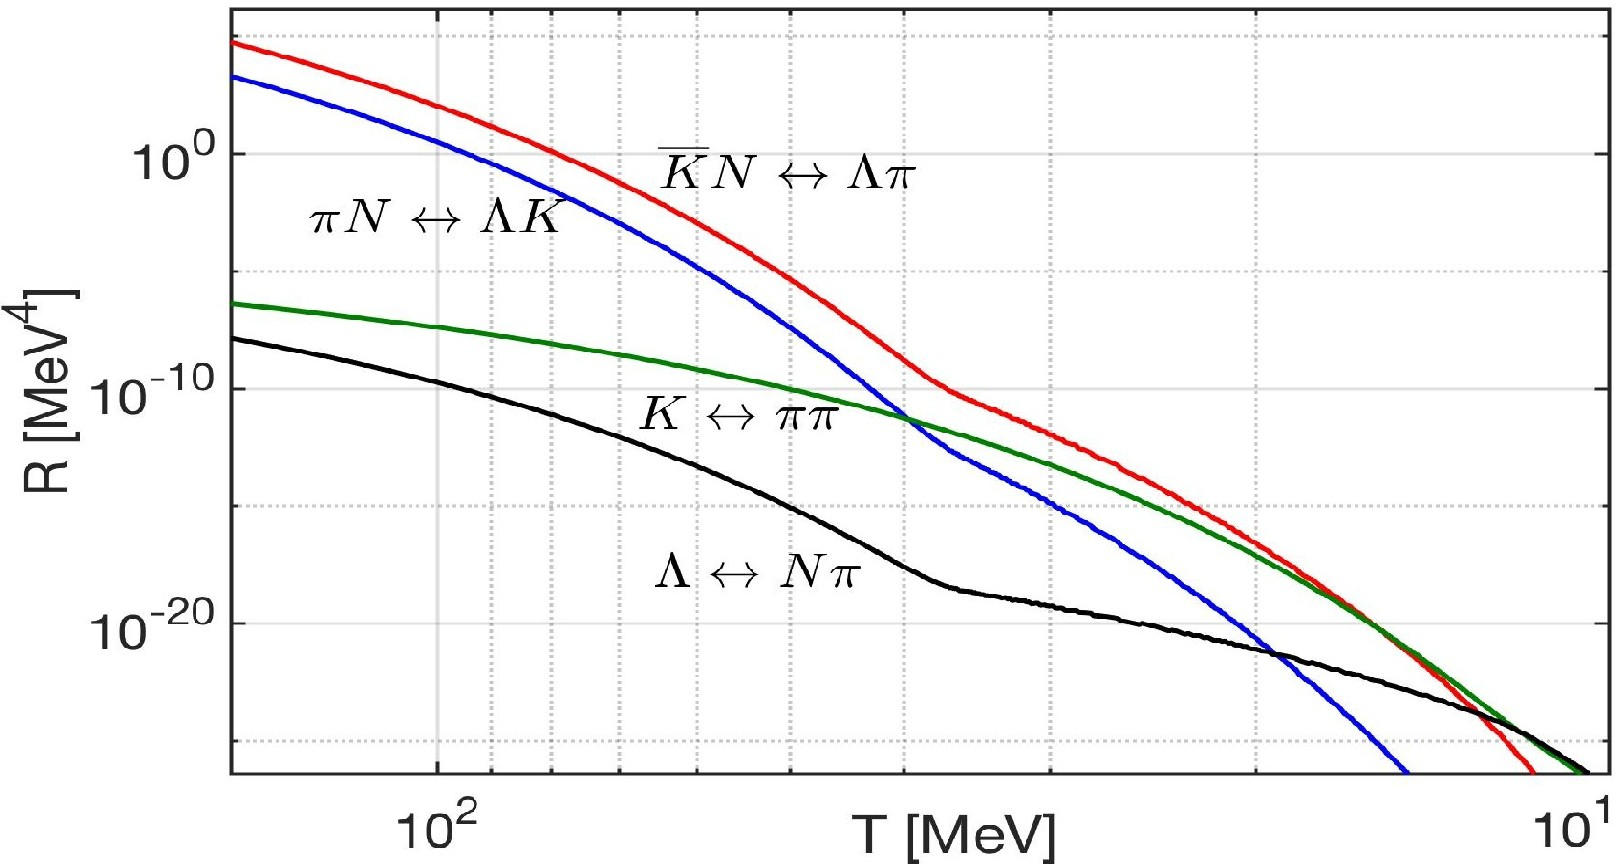
\includegraphics[width=0.9\linewidth]{./plots/NewHyperonRate_C.jpg}
\caption{\cccite{Rafelski:2023emw}, adapted from Ref.~\cite{Yang:2021bko} and thesis of C.T.Yang \cite{Yang:2024ret}. Thermal reaction rate $R$ per volume and time for important hadronic strangeness production and exchange processes as a function of temperature $150\,\mathrm{MeV}> T>10\,\mathrm{MeV}$ in the early Universe.}
\label{Lambda_Rate_volume.fig}
%\end{center}
\end{figure}
%~~~~~~~~~~~~~~~~~~~~~~~~~~~~~~~~~~~~~~~~~~~~~~~~~~~~~~~~~~~~~~~~~~~~~~~~~~~~~~

Around $T=12.9$\,MeV, the reaction $\Lambda+\pi\rightarrow\overline{K}+N$ becomes slower than the strangeness decay $\Lambda\leftrightarrow N+\pi$ and shows that at the low temperature the $\Lambda$ particles are still in equilibrium via the reaction $\Lambda\leftrightarrow N+\pi$ and little strangeness remains in the $\Lambda$. Then strangeness abundance becomes asymmetric $s\gg \bar{s}$, which implies that the assumption for strangeness conservation can only be valid until the temperature $T\sim13$\,MeV. Below this temperature a new regime opens up in which the tiny residual strangeness abundance is governed by weak decays with no re-equilibration with mesons. Also, in view of baron asymmetry, $\langle s-\bar s\rangle \ne 0$.

The primary conclusion of this first study of strangeness production and content in the early Universe, following on QGP hadronization, is that the relevant temperature domains indicate a complex interplay between baryon and meson (strange and non-strange) abundances and non-trivial decoupling from equilibrium for strange and non-strange mesons. We believe that this work contributes to the opening of a new and rich domain in the study of the Universe evolution in the future. 

%~~~~~~~~~~~~~~~~~~~~~~~~~~~~~~~~~~~~~~~~~~~~~~~~~

%{Introduction\daggerfootnote{This chapter has been published previously as \citet{Gottbrath1999}.}}


